\subsubsection{Vegetationsfilterung}

Die anschließende Filterung dient der selektiven Extraktion der Baumpunkte aus der normalisierten Gesamtpunktwolke. Zunächst werden alle Punkte mit einer HAG unter 0,8 m ausgeschlossen, um bodennahe Vegetation wie Sträucher zu eliminieren. Zudem werden alle vorklassifizierten Punkte außer den Nicht-Bodenpunkten (Klasse 20) herausgefiltert.

Zur Differenzierung der verbleibenden Vegetation von anthropogenen Strukturen werden geometrische, radiometrische und spektrale Kriterien evaluiert. Mittels einer \textit{K-Nearest-Neighbor}-Suche auf Basis der nächsten 50 Nachbarpunkte werden zunächst lokale 3D-Kovarianzmerkmale berechnet. Während ebene Strukturen wie Fassaden und Dachflächen eine hohe Planarität aufweisen, zeichnen sich zerklüftete Baumkronen durch niedrige Planaritätswerte und eine höhere Linearität infolge zahlreicher einzelner Äste aus. Ergänzend wird die Number of Returns einbezogen. Da das teiltransparente Blätterdach meist zwei oder mehr Reflexionen erzeugt, lassen sich biologische Strukturen zuverlässig von soliden Oberflächen mit nur einem Echo unterscheiden \cite{munzingerMappingUrbanForest2022}. Für die Filterung wird zudem eine Intensitätsschwelle von 140 definiert, um stark reflektierende künstliche Objekte auszuschließen \cite{zhangIndividualTreeSegmentation2024}. Abbildung \ref{fig:point-character} veranschaulicht jeweils, dass durch die Einfärbung nach der Anzahl der Rückstrahlungen (Abbildung \ref{fig:number-of-returns}) sowie nach der Intensität (Abbildung \ref{fig:intensity}) bereits in der normalisierten Punktwolke Baumstrukturen deutlich hervortreten.
\begin{figure}[htbp]
    \centering
    \begin{subfigure}[t]{0.35\columnwidth}
        \centering
        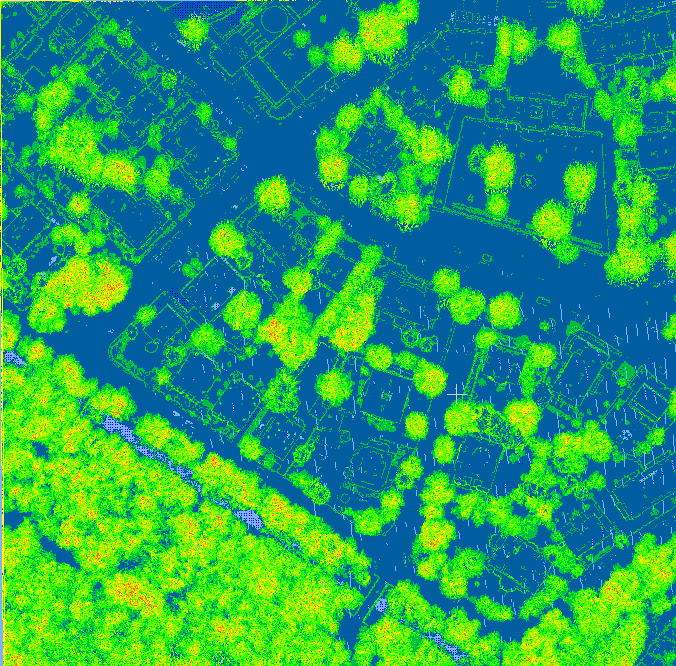
\includegraphics[width=\textwidth]{imgs/NumberOfReturns.png}
        \caption{Einfärbung nach Number of Returns}
        \label{fig:number-of-returns}
    \end{subfigure}
    \hspace{1 cm}
    \begin{subfigure}[t]{0.35\columnwidth}
        \centering
        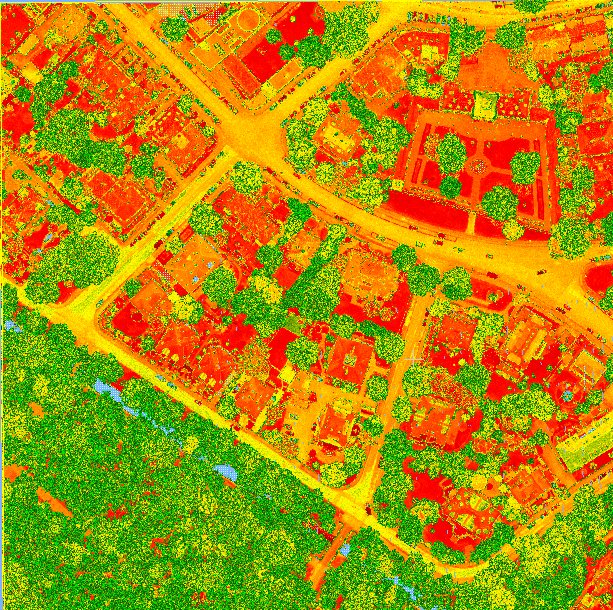
\includegraphics[width=\textwidth]{imgs/Intensitaet.png}
        \caption{Einfärbung nach Intensität}
        \label{fig:intensity}
    \end{subfigure}
    \caption[Eigenschaften der Punktwolke]{Einfärbung der normalisierten Punktwolke in CloudCompare nach Number of Returns und nach Intensität}\label{fig:point-character}
\end{figure}

Als finales spektrales Kriterium dient der NDVI, der über eine Fusion der LiDAR-Daten mit vierkanäligen DOPs berechnet wird. Da Vegetation im Bereich des NIR stark reflektiert und rotes Licht zur Photosynthese absorbiert, weisen vitale Bäume üblicherweise NDVI-Werte zwischen 0,2 und 0,8 auf. Um phänologische Variationen wie Laubabfall zu berücksichtigen, wird die Untergrenze des Filters hier auf null gesetzt \cite{munzingerMappingUrbanForest2022}. Code \ref{lst:pdal_filter} zeigt, wie diese Filterkriterien in der PDAL-Pipeline implementiert werden.
\begin{lstlisting}[label={lst:pdal_filter}, caption={[Filter]Logische Filterkriterien für die Vegetationsextraktion}, breaklines=true, breakatwhitespace=true]
{
    "type": "filters.expression",
    "expression": "(" \
        "(NumberOfReturns > 2) || " \
        "(NumberOfReturns <= 2 && Planarity < 0.6 && Linearity > 0.8)" \
        ") && (Intensity < 140) && " \
        "(Infrared + Red > 0) && " \
        "(((Infrared - Red) / (Infrared + Red)) > 0.0)"
} 

\end{lstlisting}
Zur abschließenden Bereinigung von Rauschen und Messartefakten wird ein statistischer Ausreißerfilter (\textit{Statistical Outlier Removal, \ac{SOR}}) nachgeschaltet. Dieser berechnet für jeden Punkt die mittlere Distanz zu seinen 12 nächsten Nachbarn. Punkte, deren Abstand die mittlere Distanz aller Punkte um mehr als das 1,5-fache der Standardabweichung überschreiten, werden als Ausreißer klassifiziert und über einen Range-Filter eliminiert \cite{zhangIndividualTreeSegmentation2024}. Das Resultat ist eine bereinigte Punktwolke, die ausschließlich urbane Bäume als Basis für die nachfolgende Einzelbaumsegmentierung enthält.

